\section{Grand partition function in the representation of collective variables}
The grand partition partition function is now written as 
\begin{eqnarray}
	\label{gpf_1}
	\Xi &=& \Xi_0 \int \exp \left[h \rho_0 - \frac12
	\sum\limits_{\bf k} \alpha (k) \rho_{\bf k}\rho_{-{\bf k}} \right]
	\\
	&&
	\quad{}\times
	\exp (i2\pi \sum\limits_{\bf k} \omega_{\bf k} \rho_{\bf k} + \sum_{n\ge 1} \frac{(-i2\pi)^n}{n!}\sum_{\vb{k}_1,\dotsc,\vb{k}_n} {\mathfrak M}_n(\vb{k}_1,\dotsc,\vb{k}_n) \omega_{\vb k_1}\dotsc\omega_{\vb{k}_n})
	(d\omega) (d\rho) \nonumber
\end{eqnarray}
This expression was obtained in \cite{Yukh1990} (see Eq.(2.16) therein).

The next step in calculation is to integrate over $\omega_{\vb k}$ with $\vb{k}>B$. This integration can be performed with Gaussian measure, i.e. the expressions in the exponent is restricted to the powers of $\omega$ not higher than 2. Let us denote the result of this integration by $\Xi_G$. Then the grand partition function takes the form:
\begin{equation}
	\label{Xi_as_prod}
	\Xi = \Xi_0\Xi_G\Xi_L
\end{equation}
Here $\Xi_L$ denotes long-wave contributions to the GPF and is the object of our further investigation in this paper. The expression for $\Xi_L$ is following (see also Eq.(3.5) in \cite{Yukh1990}):
\begin{eqnarray}
	\label{gpf_l1}
	\Xi_L &=& \int \exp \left[h \rho_0 - \frac12
	\sum\limits_{\vb k \atop k\le B} \alpha (k) \rho_{\vb k}\rho_{-{\vb k}} \right]
	\\
	&&
	\quad{}\times
	\exp (i2\pi \sum\limits_{\vb k \atop k\le B} \omega_{\vb k} \rho_{\vb k} + \sum_{n\ge 1} \frac{(-i2\pi)^n}{n!}\sum_{\vb{k}_1,\dotsc,\vb{k}_n \atop k_i\le B} \tilde{\frak M}_n(\vb{k}_1,\dotsc,\vb{k}_n) \omega_{\vb k_1}\dotsc\omega_{\vb{k}_n})
	(d\omega)^{N_B} (d\rho)^{N_B} \nonumber
\end{eqnarray}
Here $\tilde{\frak M}_n$ denote renormalized cumulants ${\frak M}_n$ due to integration over $k>B$ [explicity expressions are needed?], and
\begin{equation}
(d\omega)^{N_B} (d\rho)^{N_B} = \left(\prod_{\vb k\atop k\le B}d\omega_{\vb k}^c d\rho_{\vb k}^c d\omega_{\vb k}^s d\rho_{\vb k}^s \right) d\omega_0 d\rho_0
\end{equation}

In the approximation of the $4th$ basic measure density, $\Xi_L$ is expressed as:
\begin{equation}
\label{gpf_l3}
\Xi_L = \int (1 + D_4 + \frac12D_4^2 + \dotsc) W_4 (\rho;\omega) (d\rho)^{N_B}(d\omega)^{N_B}, 
\end{equation}
where the measure density $W_4(\rho; \omega)$ is
\begin{eqnarray}
	\label{meas_dens_1}
	&& W_4(\rho;\omega) = \exp \left\{ h\rho_0
	- \frac12  \sum\limits_{{\vb k}\atop k\le B} \alpha(k) \rho_{\vb k} \rho_{-{\vb k}}
	+ i2\pi \sum\limits_{{\vb k} \atop k\le B} \omega_{\vb k} \rho_{\vb k} + \right.  \nonumber\\
	&& \left.+
	\sum\limits_{n=1}^4 \frac{(-i2\pi)^n}{n!} 
	\sum\limits_{\vb{k}_1,\dotsc,\vb{k}_n\atop{k_i \le B}} \tilde{\frak M}_n(\vb{k}_1,\dotsc,\vb{k}_n)
	\omega_{{\vb k}_1} \dots \omega_{{\vb k}_n} \right\}.
\end{eqnarray}
and the following notation is introduced:
\begin{equation}
D_4 = \sum_{m>4}\frac{(-i2\pi)^m}{m!} \sum\limits_{\vb{k}_1,\dotsc,\vb{k}_m\atop{k_i \le B}}
\tilde{\frak M}_n(\vb{k}_1,\dotsc,\vb{k}_m)
\omega_{{\vb k}_1} \dots \omega_{{\vb k}_m}
\end{equation}

The quantity $N_B$ is the number of variables to be integrated over. It is equal to the
number of values that the wave vector takes on in the sphere of radius B in reciprocal space. Let's assume that the wave-vector values are distributed uniformly, then
\begin{equation}
\label{NB}
N_B = \frac{B^3}{6\pi^2}V.
\end{equation}
To derive this equation, consider the following arguments. If we had a simple cubic lattice of spacing
$c$ in real space, the first Brillouin zone of it would be a simple cubic lattice in the reciprocal
space with spacing $2B'$, where $B'=\pi/c$. The number of values taken by wave vector in this zone
would be $N_{B} = V/c^3 = V(B'/\pi)^3.$ Under our assumption, the wave vector values are distributed
uniformly. Hence, the sphere of volume $\Omega$ in reciprocal space must contain the same number of wave
vector values as a cube of the same volume $\Omega$. Since $\Omega = (2B')^3 = \frac43\pi B^3,$ one finds that $B'^3=\frac{\pi}{6}B^3$ and, therefore, arrives at Eq.~(\ref{NB}). [Some references are needed here]

In the current investigation the following approximations are to be applied.

{\it Approximation 1.} $D_4$ is neglected in the expression (\ref{gpf_l3}) for $\Xi_L$;

{\it Approximation 2.} The difference between renormalized values of cumulants $\tilde{\frak M}_n$ and original cumulants $\frak M_n$ is ignored, so that:
\begin{equation}
\tilde{\frak M}_n(\vb k^n) \approx \frak M_n(\vb k^n)
\end{equation}

{\it Approximation 3.} The dependence of cumulants $\frak M_n$ on the wave vectors $\vb k_i$ is neglected, except for the dependence via $\delta$-functions
\begin{equation}
\frak{M}_n({\vb k}^n) \approx \frak{M}_n(0^n) \delta_{\vb{k}_1 + \dotsc + \vb{k}_n}
\end{equation}
where the following notation is used for simplicity: ${\vb k}^n\equiv {\vb k}_1, \dotsc, {\vb k}_n$.

With these approximations applied, one arrives at the following expressions:
\begin{equation}
\label{gpf_l4}
\Xi_L = \int W_4 (\rho;\omega) (d\rho)^{N_B}(d\omega)^{N_B}, 
\end{equation}
and
\begin{eqnarray}
	\label{meas_dens_2}
	W_4(\rho;\omega) &=& \exp \left\{ h\rho_0
	- \frac12  \sum\limits_{{\vb k}\atop k\le B} \alpha(k) \rho_{\vb k} \rho_{-{\vb k}}
	+ i2\pi \sum\limits_{{\vb k} \atop k\le B} \omega_{\vb k} \rho_{\vb k} \right.  \nonumber\\
	&& \left.+
	\sum\limits_{n=1}^4 \frac{(-i2\pi)^n}{n!} 
	{\frak M}_n(0^n)
	\sum\limits_{\vb{k}_1,\dotsc,\vb{k}_n\atop{k_i \le B}}
	\delta_{\vb{k}_1 + \dotsc + \vb{k}_n} 
	\omega_{{\vb k}_1} \dots \omega_{{\vb k}_n} \right\}.
\end{eqnarray}
See also Eqs.~(3.12),~(3.13) in \cite{Yukh1990}.

The expression \ref{meas_dens_2} for the $4$-th measure density contains non-zero terms in all powers of $\omega$ up to 4. Let's eliminate the coefficient next to the 3-rd power in $\omega$. For this, the following change of variables is performed:
\begin{equation}
\omega_0 = \omega'_0 + \frac{\frak M_3}{(i2\pi) \frak M_4}
\end{equation}
From now on, we will understand $\frak M_n$ as $\frak{M}_n(0^n)$ where it is not ambiguous. One should remember that $\frak M_n$ are still dependent on the packing fraction $\eta$.
The 4-th measure density $W_4(\rho; \omega)$ takes the form:

\begin{eqnarray}
	\label{meas_dens_3}
	W_4(\rho;\omega) &=& \exp \left\{\frak M_0 + (h + \frak M_3/\frak M_4)\rho_0
	- \frac12  \sum\limits_{{\vb k}\atop k\le B} \alpha(k) \rho_{\vb k} \rho_{-{\vb k}}
	- i2\pi \tilde{\frak M}_1 \omega_0 + \right.  \nonumber\\
	&&
	+ i2\pi \sum\limits_{{\vb k} \atop k\le B} \omega_{\vb k} \rho_{\vb k}
	+ \frac{(-i2\pi)^2}{2!}\tilde{\frak M}_2 \sum\limits_{{\vb k} \atop k\le B} \omega_{\vb k} \omega_{-\vb k}
	\nonumber\\
	&& \left. +
	\frac{(-i2\pi)^4}{4!} 
	{\frak M}_4
	\sum\limits_{\vb{k}_1,\dotsc,\vb{k}_4\atop{k_i \le B}}
	\delta_{\vb{k}_1 + \dotsc + \vb{k}_4} 
	\omega_{{\vb k}_1} \dots \omega_{{\vb k}_4} \right\}
\end{eqnarray}
with
\begin{equation}
	\label{def:M_0}
	\frak M_0 = -\frac{\frak M_1 \frak M_3}{\frak M_4} + \frac{\frak M_2 \frak M_3^2}{2 \frak M_4^2}
	- \frac{\frak M_3^4}{8\frak M_4^3},
\end{equation}

\begin{equation}
	\label{def:tilde_M_1}
	\tilde{\frak M}_1 = \frak M_1 -\frac{\frak M_2 \frak M_3}{\frak M_4} + \frac{\frak M_3^3}{3\frak M_4^2},
\end{equation}

\begin{equation}
	\label{def:tilde_M_2}
	\tilde{\frak M}_2 = \frak M_2 - \frac{\frak M_3^2}{2 \frak M_4}.
\end{equation}
In (\ref{meas_dens_3}) the prime at $\omega_0$ is omitted.

We also want to eliminate the term at $\omega_0$. This is achieved by the change of variables
\begin{equation}
\rho_0 = \rho'_0 + \tilde{\frak M}_1.
\end{equation}
The expression for $W_4(\rho; \omega)$ becomes
\begin{eqnarray}
	\label{meas_dens_4}
	W_4(\rho;\omega) &=& \exp \left\{\tilde{\frak M}_0 + \mu^*\rho_0
	- \frac12  \sum\limits_{{\vb k}\atop k\le B} \alpha(k) \rho_{\vb k} \rho_{-{\vb k}} \right.  \nonumber\\
	&&
	+ i2\pi \sum\limits_{{\vb k} \atop k\le B} \omega_{\vb k} \rho_{\vb k}
	+ \frac{(-i2\pi)^2}{2!}\tilde{\frak M}_2 \sum\limits_{{\vb k} \atop k\le B} \omega_{\vb k} \omega_{-\vb k}
	\nonumber\\
	&& \left. +
	\frac{(-i2\pi)^4}{4!} 
	{\frak M}_4
	\sum\limits_{\vb{k}_1,\dotsc,\vb{k}_4\atop{k_i \le B}}
	\delta_{\vb{k}_1 + \dotsc + \vb{k}_4} 
	\omega_{{\vb k}_1} \dots \omega_{{\vb k}_4} \right\}
\end{eqnarray}
with
\begin{equation}
\label{tilde_frak_M0}
\tilde{\frak M}_0 = \frak M_0 + (h + {\frak M_3}/{\frak M_4})\tilde{\frak M}_1 - \frac{\alpha(0)}{2}\tilde{\frak M}_1^2
\end{equation}

\begin{equation}
	\label{mu_star}
	\mu^* = h + {\frak M_3}/{\frak M_4} + \alpha(0)\tilde{\frak M}_1
\end{equation}
In (\ref{meas_dens_4}) the prime at $\rho_0$ is omitted.

We can compare the expression~(\ref{meas_dens_4}) with Eq.~(3.14) from \cite{Yukh1990}, Eq.~(12) from \cite{YukhJSP1995}, and Eq.~(3.5) from \cite{Yukh2013}.

\begin{table}[h]
	\caption{The zero values of the cumulant $\mathfrak{M_4}$. $\mathfrak{M_4} < 0$ for $\eta_{min} < \eta < \eta_{max}$.}
	\label{tab:cum_m4_zeros}
	\begin{center}
		\begin{tabular}{|c|c|c|}
			%\begin{tabular}{cccccccccc}
			\hline
			Approximation & $\eta_{min}$ & $\eta_{max}$ \\
			\hline
			Percus-Yevick, compressibility equation~\cite{WertheimPRL1963} \quad & 0.037346 \quad & 0.221675 \quad \\
			Percus-Yevick, virial equation~\cite{ThieleJCP1963}          			& 0.037673 & 0.233899 \\
			Carnahan-Starling~\cite{CarnahanStarling1969}		& 0.037455 & 0.225572 \\
			Ree-Hoover~\cite{ReeHooverJCP1964}					& 0.037423 & 0.224260 \\
			\hline
		\end{tabular}
	\end{center}
\end{table}

\begin{figure}[htbp]
	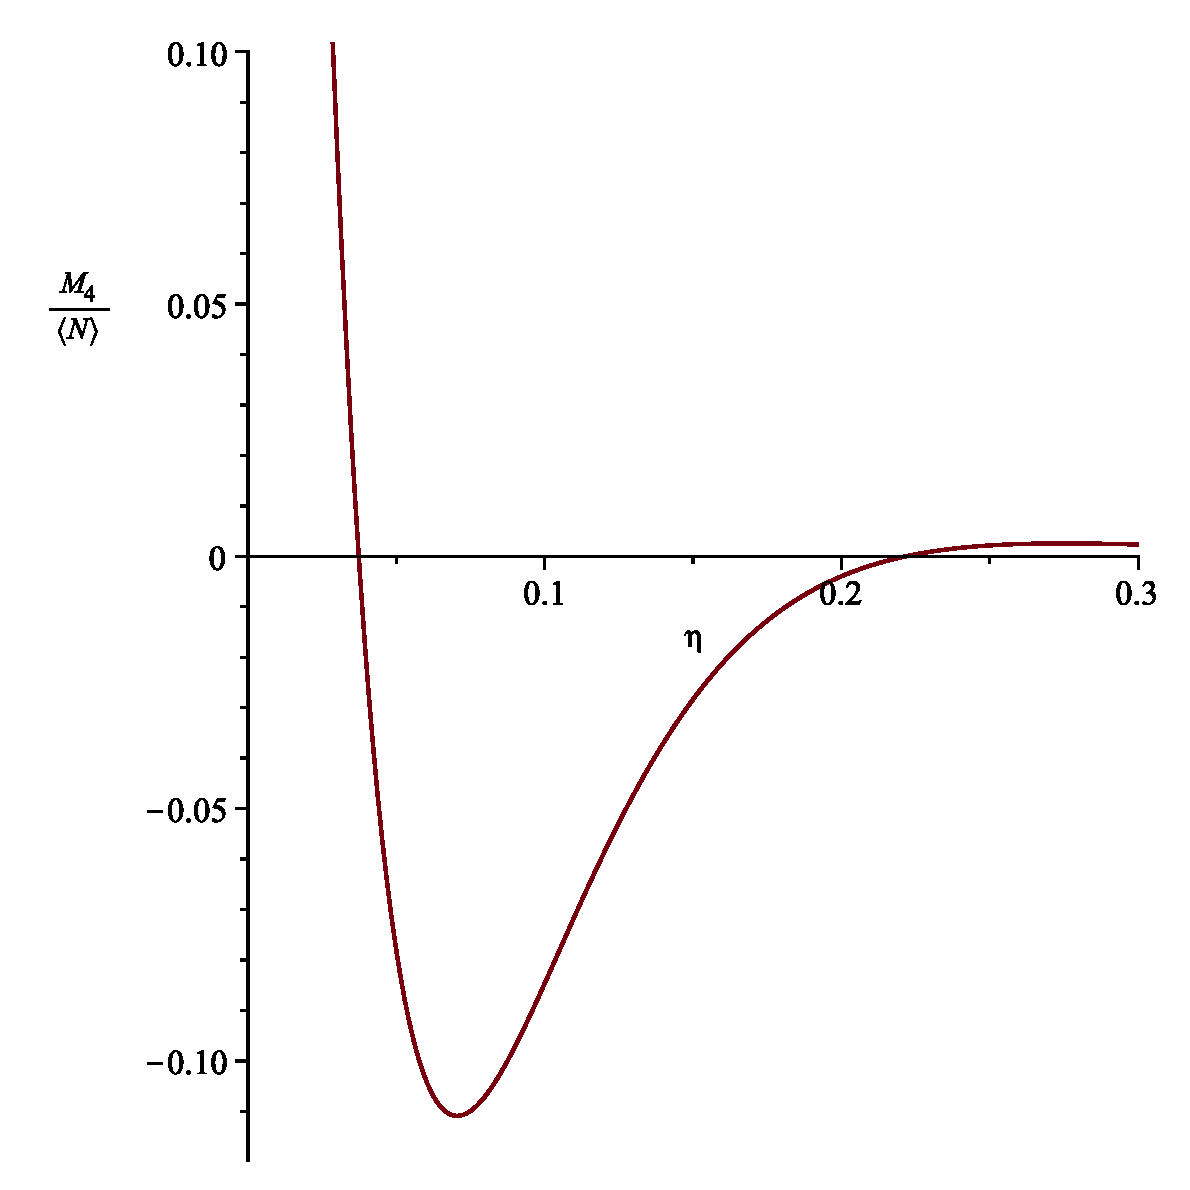
\includegraphics[width=0.7\textwidth,angle=0]{M4_at_k_equals_0_as_function_of_eta}
	\caption{Cumulant $\frak M_4$ as a function of packing fraction $\eta$ at $\vb k_i = 0$.}
	\label{m4_fig1}
\end{figure}

The first thing to note in Eq.~(\ref{meas_dens_4}) is that the integral for $\Xi_L$ in~(\ref{gpf_l4}) converges only for $\frak M_4 < 0$. The values of $\mathfrak M_4$ are negative only in some range of $\eta$. Table~{\ref{tab:cum_m4_zeros}} summarizes numerical solutions for the equation $\mathfrak{M_4}=0$ in a few approximations. Thus one can conclude that the 4-th measure density $W_4(\rho; \omega)$ is applicable only in this range of packing fraction $\eta$. We are going to work in range $0.04 \le \eta \le 0.22$. The dependence of $\frak M_4$ on $\eta$ is presented in Figure~\ref{m4_fig1}.

\subsection{Integration over $\omega$.}
Let's perform integration over $\omega$ in~(\ref{gpf_l4}), using~(\ref{meas_dens_4}) for $W_4(\rho; \omega)$. First let's single out the integral over $\omega$
\begin{eqnarray}
	J(\rho) &=& \int \exp \left(
	{\rm i}2\pi \sum\limits_{{\vb k} \atop k\le B} \omega_{\vb k} \rho_{\vb k}
	+ \frac{(-i2\pi)^2}{2!}\tilde{\frak M}_2 \sum\limits_{{\vb k} \atop k\le B} \omega_{\vb k} \omega_{-\vb k}
	\right.
	\nonumber\\
	&& \left. +
	\frac{(-i2\pi)^4}{4!} 
	{\frak M}_4
	\sum\limits_{\vb{k}_1,\dotsc,\vb{k}_4\atop{k_i \le B}}
	\delta_{\vb{k}_1 + \dotsc + \vb{k}_4} 
	\omega_{{\vb k}_1} \dots \omega_{{\vb k}_4} \right) ({\rm d} \omega)^{N_B}
\end{eqnarray}
To factorize this integral, perform the following change of variables
\begin{equation}
	\tilde{\omega}_{\vb l} = \frac{1}{\sqrt{N_B}}\sum_{\substack{\vb k \\ k \leq B}} \omega_{\vb k} {\rm e}^{-{\rm i}\vb k \vb l}
	, \quad \tilde{\rho}_{\vb l} = \frac{1}{\sqrt{N_B}} \sum_{\substack{\vb k \\ k \leq B}} \rho_{\vb k} {\rm e}^{{\rm i}\vb k \vb l}.
\end{equation}
The following relations are valid:
\begin{equation}
	\sum_{\vb l} \tilde{\omega}_{l} \tilde{\rho}_{\vb l} = \frac{1}{N_B} \sum_{\vb l} \sum_{\vb k} \omega_{\vb k} \sum_{\vb k'} \rho_{\vb k'} {\rm e}^{-{\rm i} (\vb k - \vb k') \vb l} = \sum_{\vb k} \omega_{\vb k} \rho_{\vb k},
\end{equation}
\begin{eqnarray}
	&&\sum_{\vb l}\tilde{\omega}_{\vb l}^2 = \sum_{\vb k}\omega_{\vb k} \omega_{-\vb k},
	\\
	&&N_B \sum_{\vb l}\tilde{\omega}_{\vb l}^4 = \sum\limits_{\substack{\vb{k}_1,\dotsc,\vb{k}_4 \\ {k_i \le B}}}
	\delta_{\vb{k}_1 + \dotsc + \vb{k}_4} 
	\omega_{{\vb k}_1} \dots \omega_{{\vb k}_4}
\end{eqnarray}
where the following expression for the Kronecker's $\delta$-symbol is used:
\begin{equation}
	\delta_{\vb k} = \frac{1}{N_B}\sum_{\vb l} {\rm e}^{-{\rm i} \vb k \vb l}.
\end{equation}
The sum over $\vb l$ should be understood as running over $N_B$ values in real space corresponding to the wave-vector values $\vb k, k\leq B$.

The element of integration is changed as following:
\begin{equation}
	{\rm d} \omega_0 \prod'_{\substack{\vb k \\ k\leq B}} {\rm d} \omega_{\vb k}^c {\rm d}\omega_{\vb k}^s = j \prod_{\vb l} {\rm d} \tilde{\omega}_{\vb l}
\end{equation}
where $j$ is the Jacobian of transition from $\omega_{\vb k}$ to $\tilde{\omega}_{\vb l}.$

Since the approximation of the 4-th measure density is applicable only when $\mathfrak{M_4}$ is negative, we will write the following expressions using the absolute value of this cumulant. 
Thus, the factorized expression for the integral over $\omega$ is
\begin{equation}
	J(\rho) = j\prod_{\vb l} 
	\int \exp({\rm i}2\pi \tilde{\omega}_{\vb l} \tilde{\rho}_{\vb l} - \frac{(2\pi)^2}{2} \tilde{\mathfrak{M}}_2 \tilde{\omega}_{\vb l}^2 - \frac{(2\pi)^4}{4!}N_B \abs{\mathfrak{M}_4} \tilde{\omega}_{\vb l}^4)
	{\rm d}\tilde{\omega}_{\vb l}.
\end{equation}
If we denote the integral as
\begin{equation}
	J_{\vb l}(\tilde{\rho}_{\vb l}) = \int \exp({\rm i}2\pi \tilde{\omega}_{\vb l} \tilde{\rho}_{\vb l} 
	- \frac{(2\pi)^2}{2} \tilde{\mathfrak{M}}_2 \tilde{\omega}_{\vb l}^2 - \frac{(2\pi)^4}{4!}N_B \abs{\mathfrak{M}_4} \tilde{\omega}_{\vb l}^4)
	{\rm d}\tilde{\omega}_{\vb l}
\end{equation}
then the result of integration can be presented in the following form
\begin{equation}
	J(\rho) = j\prod_{\vb l}{\rm e}^{a_0} \exp(-\sum_{n\geq 1} \frac{a_n}{n!}\tilde{\rho}_{\vb l}^n)
\end{equation}
where coefficients $a_n$ are found by the following formulae
\begin{equation}
	a_n = - \left(\frac{\partial^n \ln J_{\vb l}(\tilde{\rho}_{\vb l})}{\partial \tilde{\rho}_{\vb l}^n}\right)_{\tilde{\rho}_{\vb l}=0}.
\end{equation}

First, let's calculate ${\rm e}^{a_0}$
\begin{equation}
	Q(\tilde{\mathfrak{M}}_2, \mathfrak{M}_4) \equiv {\rm e}^{a_0} = \int_{-\infty}^{\infty} 
	\exp(- \frac{(2\pi)^2}{2} \tilde{\mathfrak{M}}_2 \tilde{\omega}_{\vb l}^2 - \frac{(2\pi)^4}{4!}N_B \abs{\mathfrak{M}_4} \tilde{\omega}_{\vb l}^4) 
	{\rm d} \tilde{\omega}_{\vb l}.
\end{equation}
Using the following representation for the Weber parabolic cylinder function $U(a,x)$
	\begin{equation}
	\label{parab_cylinder_t4}
	U(a,x) = \frac{2}{\Gamma(a+\frac{1}{2})}{\rm e}^{-\frac{x^2}{4}} \int_{0}^{\infty}t^{2a}\exp\left(-xt^2 - \frac{1}{2}t^4\right) {\rm d} t
\end{equation}
one obtains:
\begin{equation}
	\label{quantity_Q}
	Q(\tilde{\mathfrak{M}}_2, \mathfrak{M}_4) = \frac{1}{2\sqrt{\pi}} \left(\frac{12}{N_B \abs{\mathfrak{M}_4}}\right)^{1/4} {\rm e}^{y^2/2} U(0,y)
\end{equation}
where 
\begin{equation}
	y = \left( \frac{3 \tilde{\mathfrak{M}_2^2}}{N_B \abs{\mathfrak{M}_4}}\right)^{1/2}.
\end{equation}

Now, let's calculate $a_2$.

For $a_2$ the result is
\begin{equation}
	a_2 = \left(\frac{3}{N_B \abs{\mathfrak{M}_4}}\right)^{1/2} U(y),
\end{equation}
where 
\begin{equation}
	U(y) = \frac{U(1,y)}{U(0,y)}.
\end{equation}

For $a_4$ the result is
\begin{equation}
	a_4 = \frac{3}{N_B \abs{\mathfrak{M}_4}}\left(3U^2(y) -3 \frac{U(2,y)}{U(0,y)}\right) = 
	\frac{3}{N_B \abs{\mathfrak{M}_4}} \phi(y)
\end{equation}
where 
\begin{equation}
	\phi(y) = 3U^2(y) + 2yU(y) - 2.
\end{equation}
In the above equation we used the following recurrence relation for the parabolic cylinder function $U$:
\begin{equation}
	3U(2,y) = -2yU(1,y) + 2U(0,y).
\end{equation}

The quantity $J(\rho)$ takes the form
\begin{equation}
	J(\rho) = j Q(\tilde{\mathfrak{M}_2}, \mathfrak{M}_4)^{N_B}
	\exp(-\frac{a_2}{2}\sum_{\substack{\vb k \\ k \leq B}} \rho_{\vb k}\rho_{-{\vb k}} 
	- \frac{a_4}{N_B 4!} \sum_{\substack{\vb k_1, \dotsc, \vb k_4 \\ k_i \leq B}} \rho_{\vb k_1} \dotsc \rho_{\vb k_4} \delta_{\vb{k}_1 + \dotsc + \vb{k}_4} )
\end{equation}
where the following equations were taken into account
\begin{eqnarray}
	&&\sum_{\vb l}\tilde{\rho}_{\vb l}^2 = \sum_{\vb k}\rho_{\vb k} \rho_{-\vb k},
	\\
	&&\sum_{\vb l}\tilde{\rho}_{\vb l}^4 = \frac{1}{N_B}\sum\limits_{\substack{\vb{k}_1,\dotsc,\vb{k}_4 \\ {k_i \le B}}}
	\delta_{\vb{k}_1 + \dotsc + \vb{k}_4} 
	\rho_{{\vb k}_1} \dots \rho_{{\vb k}_4}
\end{eqnarray}

Finally, the quantity $\Xi_L$ takes the form
\begin{equation}
	\label{Xi_L}
	\Xi_L = jQ(\tilde{\mathfrak{M}_2}, \mathfrak{M}_4)^{N_B} \exp(\tilde{\mathfrak{M}}_0) \Xi_L^{(1)}
\end{equation}
where $Q(\tilde{\mathfrak{M}_2}, \mathfrak{M}_4)$ is given by~(\ref{quantity_Q}), $N_B$ by~(\ref{NB}), $\tilde{\mathfrak{M}_0}$ by~(\ref{tilde_frak_M0}), and $\Xi_L^{(1)}$ is defined as follows
\begin{equation}
	\label{Xi_L_1}
	\Xi_L^{(1)} = \int \exp(\mu^* \rho_0 - \frac{1}{2} \sum_{\substack{\vb k \\ k \leq B}} d(k) \rho_{\vb k} \rho_{-\vb k} - \frac{a_4}{4! N_B} \sum_{\substack{\vb k_1, \dotsc, \vb k_4 \\ k_i \leq B}} \rho_{\vb k_1} \dotsc \rho_{\vb k_4} \delta_{\vb{k}_1 + \dotsc + \vb{k}_4} ) ({\rm d} \rho)^{N_B}
\end{equation}
where $\mu^*$ is given by~(\ref{mu_star}), and 
\begin{equation}
	d(k) = a_2 + \alpha(k),
\end{equation}
where $\alpha(k)$ is given by~(\ref{def:h}).

\subsection{Coefficients of the effective Hamiltonian}
The argument $y$ of functions entering different expressions in the previous subsection is itself a function of $\eta$ and $B\sigma$. Let's show this.
\begin{equation}
	y=\left(\frac{3\tilde{\mathfrak{M}}_2^2}{N_B \abs{\mathfrak{M}_4}}\right)^{1/2} = \left(\frac{\langle N \rangle_0}{N_B}\right)^{1/2} \left(\frac{3\tilde{\mathfrak{m}}_2^2}{\abs{\mathfrak{m}_4}}\right)^{1/2},
\end{equation}
where the following notation is introduced
\begin{equation}
	\tilde{\mathfrak{m}}_2 = \mathfrak{m}_2 - \frac{\mathfrak{m}_3^2}{2\mathfrak{m}_4}.
\end{equation}
In the expression for $y$ the second multiplier depends only on $\eta$. Let's take a look at the first multiplier. Taking into account~(\ref{NB}), one has
\begin{equation}
	\frac{\langle N \rangle_0}{N_B} = \frac{\langle N \rangle_0}{V} \frac{6\pi^2}{B^3} = \frac{\langle N \rangle_0}{V}\sigma^3 \frac{6\pi^2}{(B\sigma)^3} = \frac{\pi}{6}\frac{\langle N \rangle_0}{V}\sigma^3 \frac{36\pi}{(B\sigma)^3} = \eta \frac{36\pi}{(B\sigma)^3}.
\end{equation}
The quantity $B\sigma$ is dimensionless but ist value depends on how $B$ is selected. Based on the previous works [References are needed], the condition for selecting $B$ is $\hat{\Phi}_{k=B} = 0.$ This condition impose some restrictions on the attractive part of the interaction potential, in particular that $\hat{\Phi}_0 < 0.$ However, section of the potential in the form of Eq.~(\ref{short-range-potential}) obeys this condition very well. 

The explicit expression for the Fourier component of such potential is the following
\begin{eqnarray}
	\hat{\Phi}_k &=& -16\pi \varepsilon \alpha^3 
	\left\{
		\frac{1}{1+k^2\alpha^2}\left(\frac{\sigma}{\alpha} + \frac{2}{1+k^2\alpha^2}\right) \cos(k\sigma)
	\right.
	\nonumber\\
	&& \left.
	 -\frac{1}{4 + k^2\alpha^2} \left(\frac{\sigma}{\alpha} + \frac{4}{4 + k^2\alpha^2}\right) \cos(k\sigma)
	 \right.
	 \nonumber \\
	&& \left.
	+ \frac{\sigma/\alpha}{1 + k^2\alpha^2} \left(\frac{\sigma}{\alpha} + \frac{1 - k^2\alpha^2}{1 + k^2 \alpha^2}\right) \frac{\sin(k\sigma)}{k\sigma}
	\right.
	\nonumber\\
	&& \left.
	- \frac{\sigma/\alpha}{4 + k^2\alpha^2} \left(2\frac{\sigma}{\alpha} + \frac{4 - k^2\alpha^2}{4 + k^2\alpha^2}\right) \frac{\sin(k\sigma)}{k\sigma}
	\right\}.
\end{eqnarray}
In this expression it is already taken into account that
\begin{equation}
	\sigma = R_0 - \alpha\ln(2).
\end{equation}

\begin{figure}[htbp]
	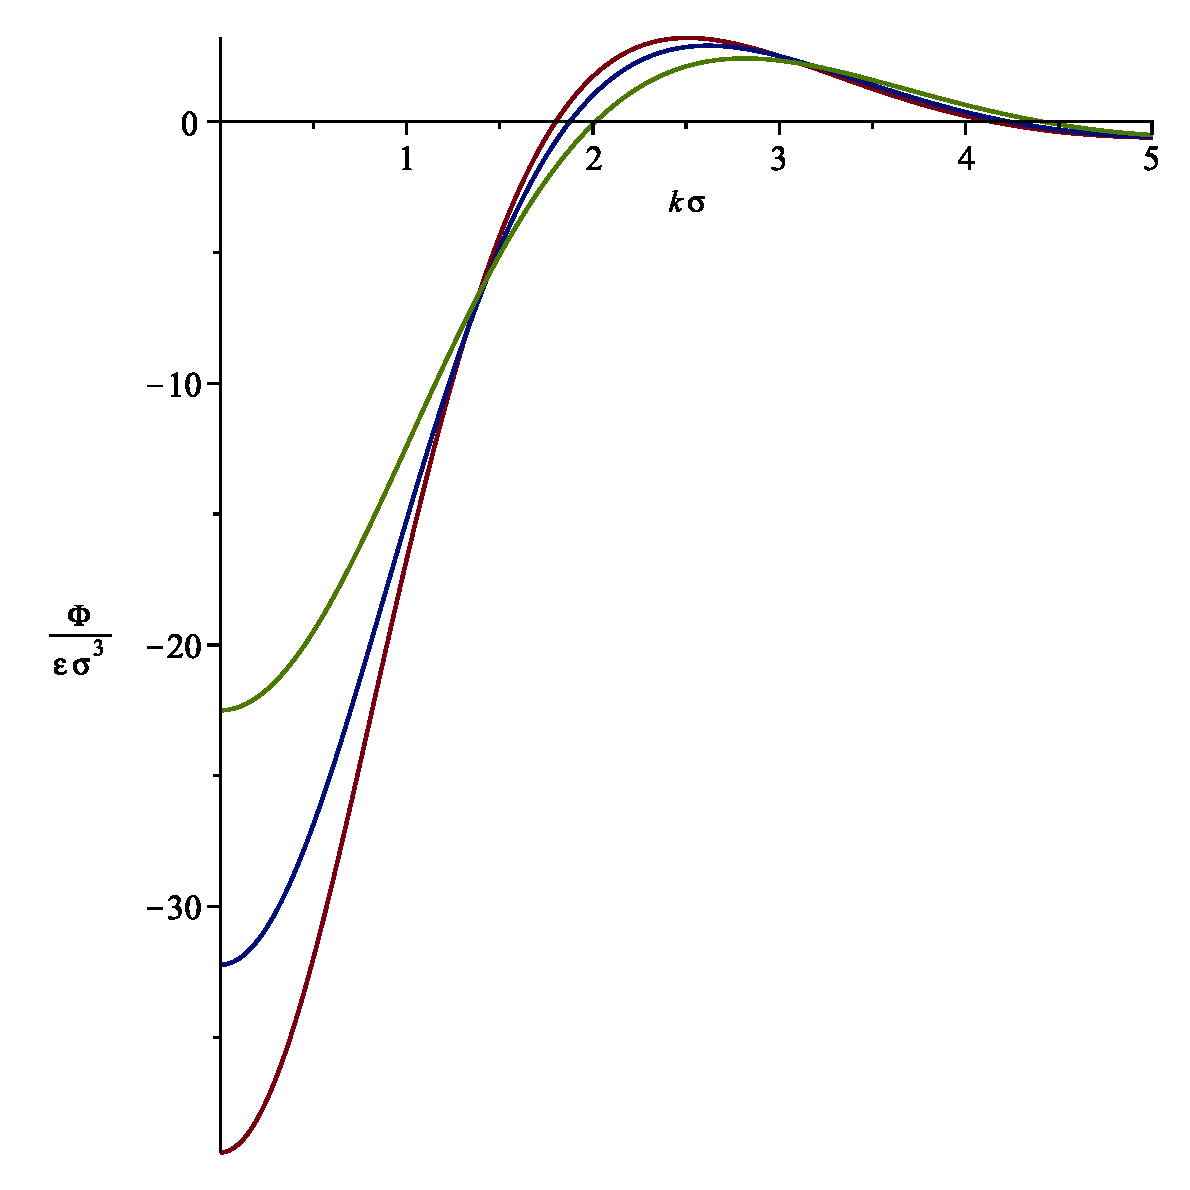
\includegraphics[width=0.45\textwidth,angle=0]{fourier_for_different_parameter_values} \hfill
	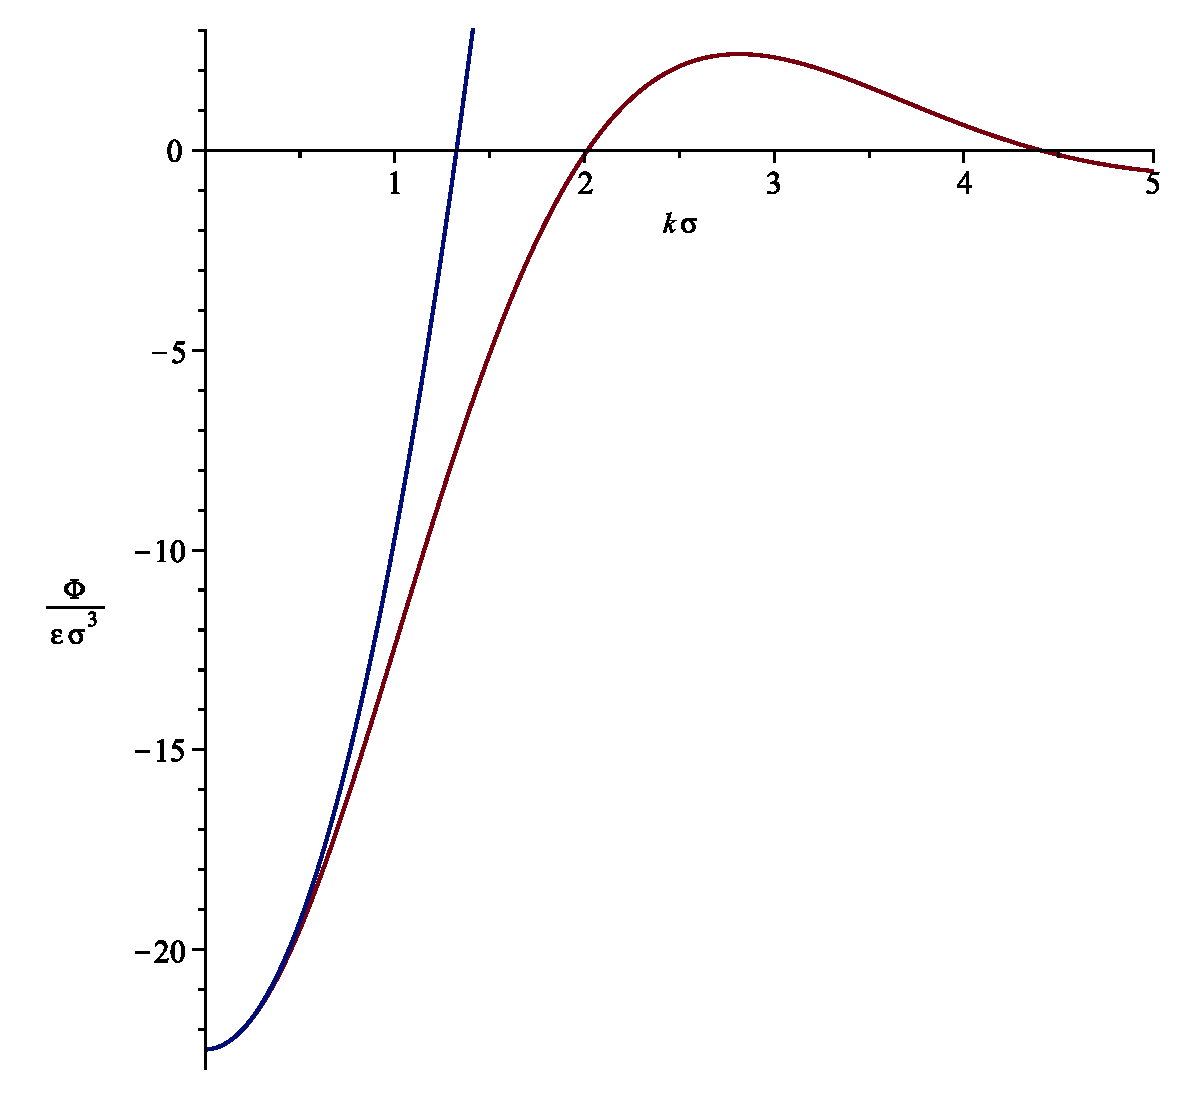
\includegraphics[width=0.45\textwidth,angle=0]{fourier_and_parabolic_potential} \\
	\parbox{0.5\textwidth}{\caption{\label{fig:fourier_for_some_parameter_values} Fourier component of the attractive part of interaction potential for different values of $R_0/\alpha$. 1 - $2.77$, 2 - 3.0, 3 - 3.5.
	}} \hfill
	\parbox{0.45\textwidth}{\caption{\label{fig:fourier_and_parabolic} Fourier component of the attractive part of interaction potential for $R_0/\alpha=3.5$ and corresponding parabolic approximation.
	}}
\end{figure}

\begin{table}[h]
	\caption{The zero values $B\sigma$ and parameters of the parabolic approximation of the Fourier component $\hat{\Phi}_{k}$ for different values of $R_0/\alpha$.}
	\label{tab:potential_fourier_zeros}
	\begin{center}
		\begin{tabular}{|c|c|c|c|}
			%\begin{tabular}{cccccccccc}
			\hline
			$R_0/\alpha$ \quad & $B\sigma$ \quad & $2b^2$ \quad & $ \frac{1}{\sqrt{2}b}$ \quad \\
			\hline
			2.0  & 1.47 & 1.68 & 0.77 \\
			2.5  & 1.70 & 1.02 & 0.99 \\
			3.0  & 1.88 & 0.72 & 1.18 \\
			3.5  & 2.01 & 0.57 & 1.33 \\
			4.0  & 2.13 & 0.48 & 1.45 \\
			4.5  & 2.22 & 0.42 & 1.55 \\
			5.0  & 2.29 & 0.37 & 1.64 \\
			\hline
		\end{tabular}
	\end{center}
\end{table}

In Figure~\ref{fig:fourier_for_some_parameter_values} the dependence of $\hat{\Phi}_k/(\varepsilon\sigma^3)$ on $k\sigma$ is shown for a few values of parameter $R_0/\alpha$. Values of $B\sigma$ for different $R_0/\alpha$ are presented in Table~\ref{tab:potential_fourier_zeros}

In some particular calculations further on, the following approximation will be used for the Fourier transform at $k<B$
\begin{equation}
	\hat{\Phi}_k = \hat{\Phi}_0(1 - 2b^2k^2)
\end{equation}
where 
\begin{equation}
	2b^2 = -\frac{1}{2\hat{\Phi}_0} \frac{\partial^2 \hat{\Phi}_k}{\partial k^2} \bigg|_{k=0}.
\end{equation}
Values of $2b^2$ along with $1/(\sqrt{2}b)$ (the point at which the parabolic approximation is equal to zero) are also presented in Table~\ref{tab:potential_fourier_zeros}. Figure~\ref{fig:fourier_and_parabolic} shows $\hat{\Phi}_k$ together with its parabolic approximation in one picture.

At this point we can build some graphics for coefficients $a_2$ and $a_4$ as functions of $\eta$.
First, for $a_2$ one has
\begin{equation}
	a_2 = \left(\frac{3}{N_B \langle N \rangle_0 \abs{\mathfrak{m}_4}}\right)^{1/2} U(y) 
	= \frac{1}{\langle N \rangle_0} \left(\frac{\langle N \rangle_0}{N_B}\right)^{1/2} \left(\frac{3}{\abs{\mathfrak{m}_4}}\right)^{1/2} U(y)
\end{equation}
and from here it is seen that the quantity $\langle N \rangle_0 a_2$ depends only on $\eta$ and the parameter $B\sigma$ of the interaction potential, see Figure~\ref{fig:a2_vs_eta}

For $a_4$ one has
\begin{equation}
	a_4 = \frac{3}{N_B \langle N \rangle_0 \abs{\mathfrak{m}_4}} \phi(y) = \frac{1}{\langle N \rangle_0^2} \frac{\langle N \rangle_0}{N_B} \frac{3}{\abs{\mathfrak{m}_4}} \phi(y)
\end{equation}
and from here it is seen that the quantity $\langle N \rangle_0^2 a_4$ depends only on $\eta$ and the parameter $B\sigma$ of the interaction potential, see Figure~\ref{fig:a4_vs_eta}

\begin{figure}[htbp]
	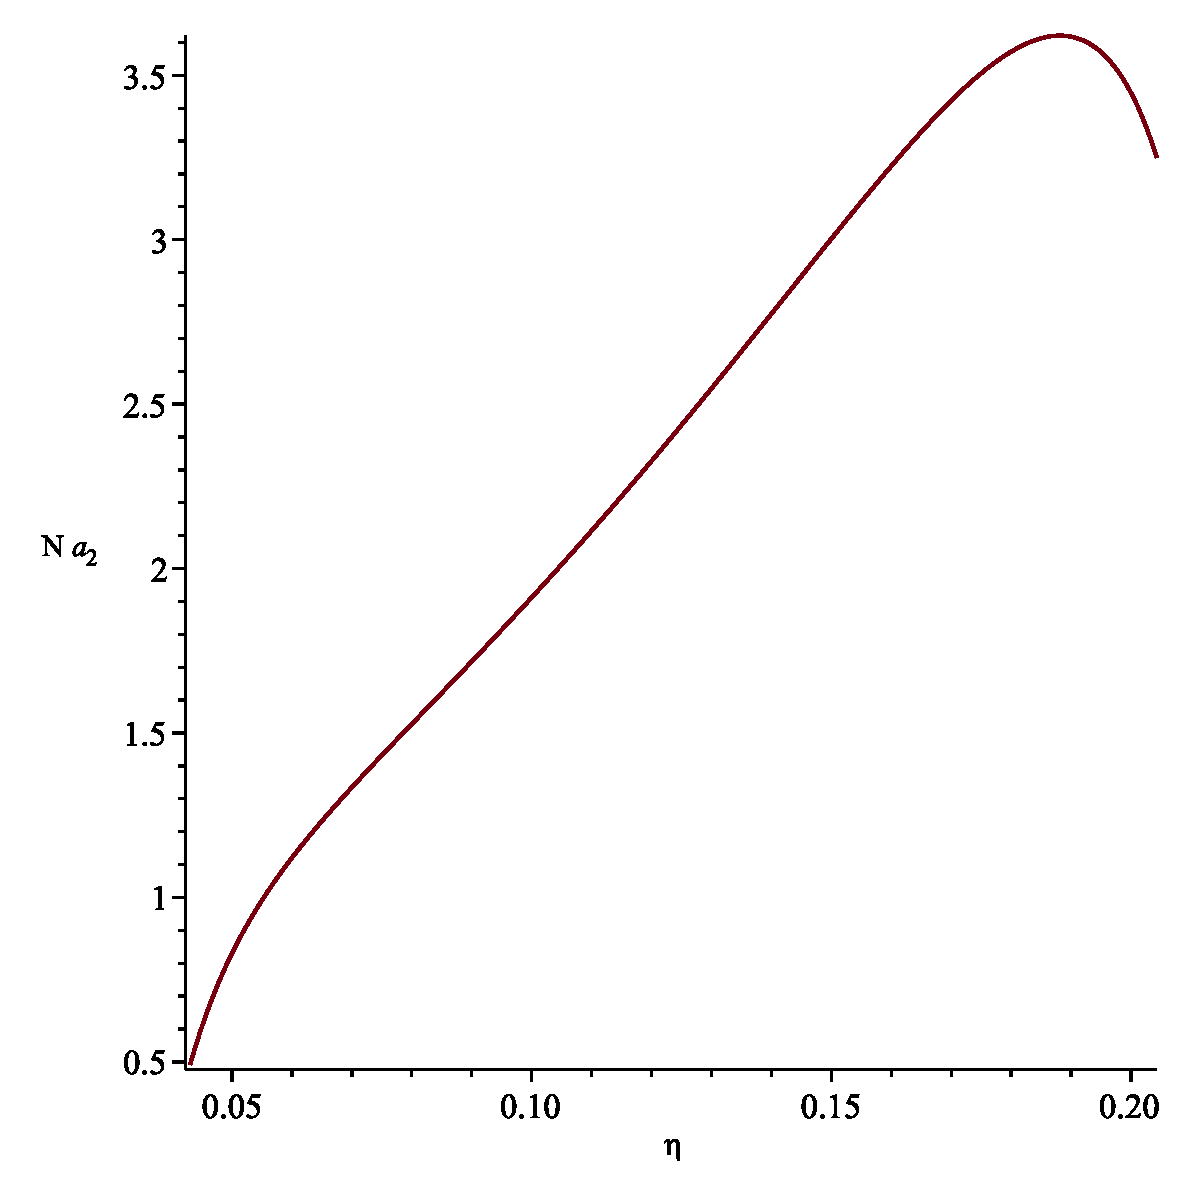
\includegraphics[width=0.45\textwidth,angle=0]{a2_as_function_of_eta} \hfill
	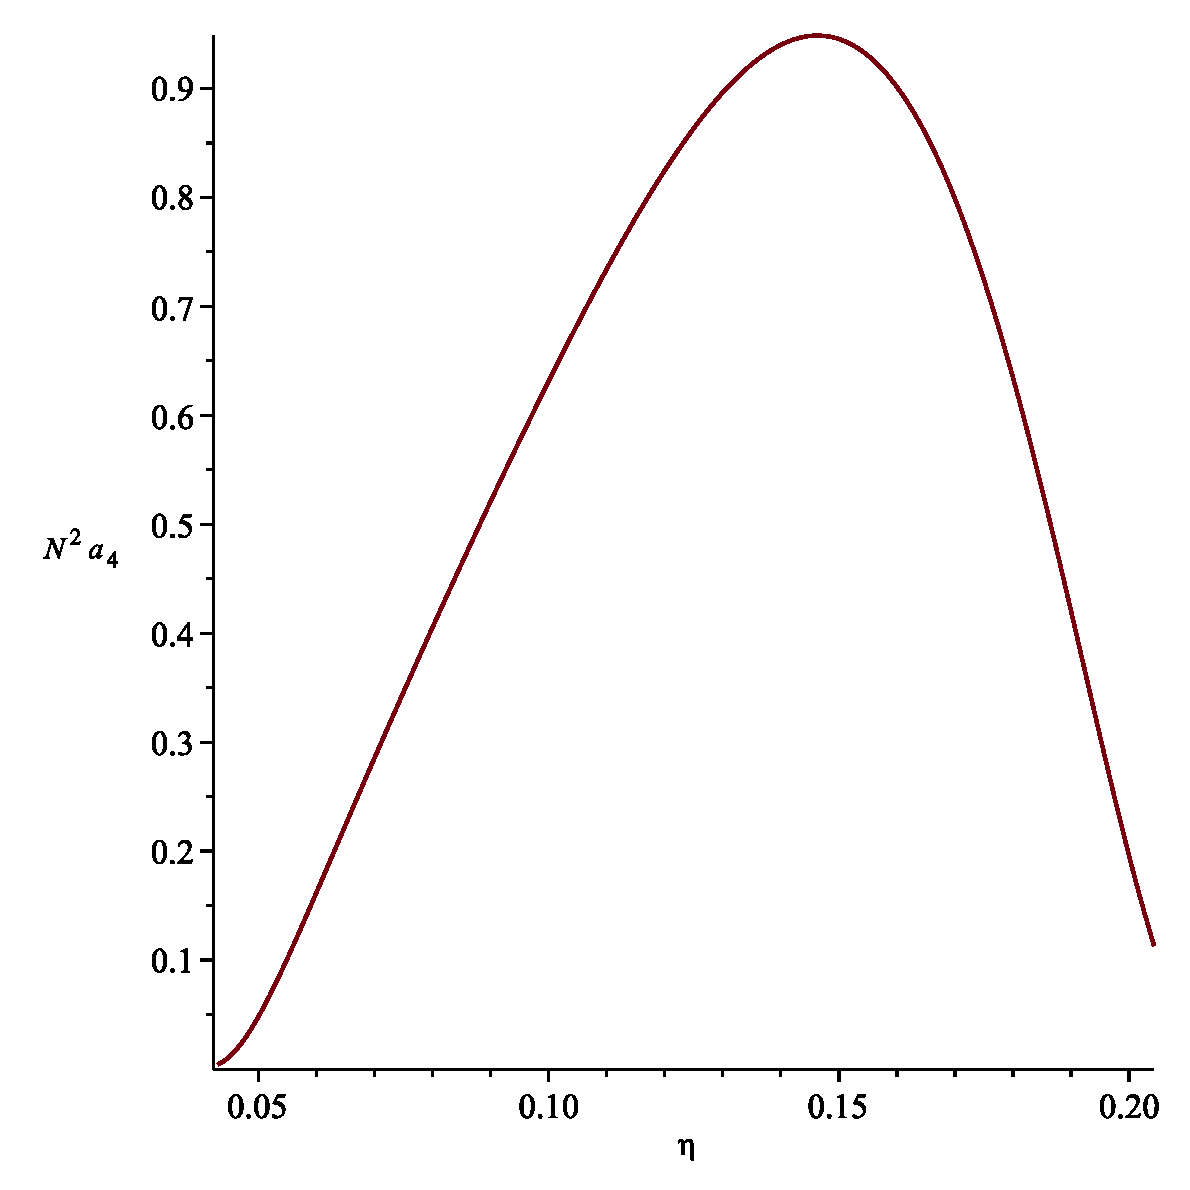
\includegraphics[width=0.45\textwidth,angle=0]{a4_as_function_of_eta} \\
	\parbox{0.5\textwidth}{\caption{\label{fig:a2_vs_eta} Quantity $\langle N \rangle_0 a_2$ as a function of $\eta$ for $R_0/\alpha=3.5$.
	}} \hfill
	\parbox{0.45\textwidth}{\caption{\label{fig:a4_vs_eta} Quantity $\langle N \rangle_0^2 a_4$ as a function of $\eta$ for $R_0/\alpha=3.5$.
	}}
\end{figure}

To rewrite $d(k)$ in a useful form, let's first consider the quantity $\alpha(k)$
\begin{equation}
	\alpha(k) = \frac{\beta \hat{\Phi}_k}{V} = \frac{1}{\langle N \rangle_0} \frac{6}{\pi}\eta \frac{\varepsilon}{k_B T} \frac{\hat{\Phi}_k}{\varepsilon\sigma^3}.
\end{equation}
It is seen now that the quantity $\langle N \rangle_0 d(k)$ is a function of $\eta$, but also depends on the parameter of the interaction potential $\Phi$, as well as on the temperature $T$. 